\documentclass[11pt]{article}

    \usepackage[breakable]{tcolorbox}
    \usepackage{parskip} % Stop auto-indenting (to mimic markdown behaviour)
    

    % Basic figure setup, for now with no caption control since it's done
    % automatically by Pandoc (which extracts ![](path) syntax from Markdown).
    \usepackage{graphicx}
    % Keep aspect ratio if custom image width or height is specified
    \setkeys{Gin}{keepaspectratio}
    % Maintain compatibility with old templates. Remove in nbconvert 6.0
    \let\Oldincludegraphics\includegraphics
    % Ensure that by default, figures have no caption (until we provide a
    % proper Figure object with a Caption API and a way to capture that
    % in the conversion process - todo).
    \usepackage{caption}
    \DeclareCaptionFormat{nocaption}{}
    \captionsetup{format=nocaption,aboveskip=0pt,belowskip=0pt}

    \usepackage{float}
    \floatplacement{figure}{H} % forces figures to be placed at the correct location
    \usepackage{xcolor} % Allow colors to be defined
    \usepackage{enumerate} % Needed for markdown enumerations to work
    \usepackage{geometry} % Used to adjust the document margins
    \usepackage{amsmath} % Equations
    \usepackage{amssymb} % Equations
    \usepackage{textcomp} % defines textquotesingle
    % Hack from http://tex.stackexchange.com/a/47451/13684:
    \AtBeginDocument{%
        \def\PYZsq{\textquotesingle}% Upright quotes in Pygmentized code
    }
    \usepackage{upquote} % Upright quotes for verbatim code
    \usepackage{eurosym} % defines \euro

	\input{../../macros.tex}
    \usepackage{iftex}
    \ifPDFTeX
        \usepackage[T1]{fontenc}
        \IfFileExists{alphabeta.sty}{
              \usepackage{alphabeta}
          }{
              \usepackage[mathletters]{ucs}
              \usepackage[utf8x]{inputenc}
          }
    \else
        \usepackage{fontspec}
        \usepackage{unicode-math}
    \fi

    \usepackage{fancyvrb} % verbatim replacement that allows latex
    \usepackage{grffile} % extends the file name processing of package graphics
                         % to support a larger range
    \makeatletter % fix for old versions of grffile with XeLaTeX
    \@ifpackagelater{grffile}{2019/11/01}
    {
      % Do nothing on new versions
    }
    {
      \def\Gread@@xetex#1{%
        \IfFileExists{"\Gin@base".bb}%
        {\Gread@eps{\Gin@base.bb}}%
        {\Gread@@xetex@aux#1}%
      }
    }
    \makeatother
    \usepackage[Export]{adjustbox} % Used to constrain images to a maximum size
    \adjustboxset{max size={0.9\linewidth}{0.9\paperheight}}

    % The hyperref package gives us a pdf with properly built
    % internal navigation ('pdf bookmarks' for the table of contents,
    % internal cross-reference links, web links for URLs, etc.)
    \usepackage{hyperref}
    % The default LaTeX title has an obnoxious amount of whitespace. By default,
    % titling removes some of it. It also provides customization options.
    \usepackage{titling}
    \usepackage{longtable} % longtable support required by pandoc >1.10
    \usepackage{booktabs}  % table support for pandoc > 1.12.2
    \usepackage{array}     % table support for pandoc >= 2.11.3
    \usepackage{calc}      % table minipage width calculation for pandoc >= 2.11.1
    \usepackage[inline]{enumitem} % IRkernel/repr support (it uses the enumerate* environment)
    \usepackage[normalem]{ulem} % ulem is needed to support strikethroughs (\sout)
                                % normalem makes italics be italics, not underlines
    \usepackage{soul}      % strikethrough (\st) support for pandoc >= 3.0.0
    \usepackage{mathrsfs}
    
    
    % Colors for the hyperref package
    \definecolor{urlcolor}{rgb}{0,.145,.698}
    \definecolor{linkcolor}{rgb}{.71,0.21,0.01}
    \definecolor{citecolor}{rgb}{.12,.54,.11}

    % ANSI colors
    \definecolor{ansi-black}{HTML}{3E424D}
    \definecolor{ansi-black-intense}{HTML}{282C36}
    \definecolor{ansi-red}{HTML}{E75C58}
    \definecolor{ansi-red-intense}{HTML}{B22B31}
    \definecolor{ansi-green}{HTML}{00A250}
    \definecolor{ansi-green-intense}{HTML}{007427}
    \definecolor{ansi-yellow}{HTML}{DDB62B}
    \definecolor{ansi-yellow-intense}{HTML}{B27D12}
    \definecolor{ansi-blue}{HTML}{208FFB}
    \definecolor{ansi-blue-intense}{HTML}{0065CA}
    \definecolor{ansi-magenta}{HTML}{D160C4}
    \definecolor{ansi-magenta-intense}{HTML}{A03196}
    \definecolor{ansi-cyan}{HTML}{60C6C8}
    \definecolor{ansi-cyan-intense}{HTML}{258F8F}
    \definecolor{ansi-white}{HTML}{C5C1B4}
    \definecolor{ansi-white-intense}{HTML}{A1A6B2}
    \definecolor{ansi-default-inverse-fg}{HTML}{FFFFFF}
    \definecolor{ansi-default-inverse-bg}{HTML}{000000}

    % common color for the border for error outputs.
    \definecolor{outerrorbackground}{HTML}{FFDFDF}

    % commands and environments needed by pandoc snippets
    % extracted from the output of `pandoc -s`
    \providecommand{\tightlist}{%
      \setlength{\itemsep}{0pt}\setlength{\parskip}{0pt}}
    \DefineVerbatimEnvironment{Highlighting}{Verbatim}{commandchars=\\\{\}}
    % Add ',fontsize=\small' for more characters per line
    \newenvironment{Shaded}{}{}
    \newcommand{\KeywordTok}[1]{\textcolor[rgb]{0.00,0.44,0.13}{\textbf{{#1}}}}
    \newcommand{\DataTypeTok}[1]{\textcolor[rgb]{0.56,0.13,0.00}{{#1}}}
    \newcommand{\DecValTok}[1]{\textcolor[rgb]{0.25,0.63,0.44}{{#1}}}
    \newcommand{\BaseNTok}[1]{\textcolor[rgb]{0.25,0.63,0.44}{{#1}}}
    \newcommand{\FloatTok}[1]{\textcolor[rgb]{0.25,0.63,0.44}{{#1}}}
    \newcommand{\CharTok}[1]{\textcolor[rgb]{0.25,0.44,0.63}{{#1}}}
    \newcommand{\StringTok}[1]{\textcolor[rgb]{0.25,0.44,0.63}{{#1}}}
    \newcommand{\CommentTok}[1]{\textcolor[rgb]{0.38,0.63,0.69}{\textit{{#1}}}}
    \newcommand{\OtherTok}[1]{\textcolor[rgb]{0.00,0.44,0.13}{{#1}}}
    \newcommand{\AlertTok}[1]{\textcolor[rgb]{1.00,0.00,0.00}{\textbf{{#1}}}}
    \newcommand{\FunctionTok}[1]{\textcolor[rgb]{0.02,0.16,0.49}{{#1}}}
    \newcommand{\RegionMarkerTok}[1]{{#1}}
    \newcommand{\ErrorTok}[1]{\textcolor[rgb]{1.00,0.00,0.00}{\textbf{{#1}}}}
    \newcommand{\NormalTok}[1]{{#1}}

    % Additional commands for more recent versions of Pandoc
    \newcommand{\ConstantTok}[1]{\textcolor[rgb]{0.53,0.00,0.00}{{#1}}}
    \newcommand{\SpecialCharTok}[1]{\textcolor[rgb]{0.25,0.44,0.63}{{#1}}}
    \newcommand{\VerbatimStringTok}[1]{\textcolor[rgb]{0.25,0.44,0.63}{{#1}}}
    \newcommand{\SpecialStringTok}[1]{\textcolor[rgb]{0.73,0.40,0.53}{{#1}}}
    \newcommand{\ImportTok}[1]{{#1}}
    \newcommand{\DocumentationTok}[1]{\textcolor[rgb]{0.73,0.13,0.13}{\textit{{#1}}}}
    \newcommand{\AnnotationTok}[1]{\textcolor[rgb]{0.38,0.63,0.69}{\textbf{\textit{{#1}}}}}
    \newcommand{\CommentVarTok}[1]{\textcolor[rgb]{0.38,0.63,0.69}{\textbf{\textit{{#1}}}}}
    \newcommand{\VariableTok}[1]{\textcolor[rgb]{0.10,0.09,0.49}{{#1}}}
    \newcommand{\ControlFlowTok}[1]{\textcolor[rgb]{0.00,0.44,0.13}{\textbf{{#1}}}}
    \newcommand{\OperatorTok}[1]{\textcolor[rgb]{0.40,0.40,0.40}{{#1}}}
    \newcommand{\BuiltInTok}[1]{{#1}}
    \newcommand{\ExtensionTok}[1]{{#1}}
    \newcommand{\PreprocessorTok}[1]{\textcolor[rgb]{0.74,0.48,0.00}{{#1}}}
    \newcommand{\AttributeTok}[1]{\textcolor[rgb]{0.49,0.56,0.16}{{#1}}}
    \newcommand{\InformationTok}[1]{\textcolor[rgb]{0.38,0.63,0.69}{\textbf{\textit{{#1}}}}}
    \newcommand{\WarningTok}[1]{\textcolor[rgb]{0.38,0.63,0.69}{\textbf{\textit{{#1}}}}}
    \makeatletter
    \newsavebox\pandoc@box
    \newcommand*\pandocbounded[1]{%
      \sbox\pandoc@box{#1}%
      % scaling factors for width and height
      \Gscale@div\@tempa\textheight{\dimexpr\ht\pandoc@box+\dp\pandoc@box\relax}%
      \Gscale@div\@tempb\linewidth{\wd\pandoc@box}%
      % select the smaller of both
      \ifdim\@tempb\p@<\@tempa\p@
        \let\@tempa\@tempb
      \fi
      % scaling accordingly (\@tempa < 1)
      \ifdim\@tempa\p@<\p@
        \scalebox{\@tempa}{\usebox\pandoc@box}%
      % scaling not needed, use as it is
      \else
        \usebox{\pandoc@box}%
      \fi
    }
    \makeatother

    % Define a nice break command that doesn't care if a line doesn't already
    % exist.
    \def\br{\hspace*{\fill} \\* }
    % Math Jax compatibility definitions
    \def\gt{>}
    \def\lt{<}
    \let\Oldtex\TeX
    \let\Oldlatex\LaTeX
    \renewcommand{\TeX}{\textrm{\Oldtex}}
    \renewcommand{\LaTeX}{\textrm{\Oldlatex}}
    % Document parameters
    % Document title
    \title{Homework\_09}
    
    
    
    
    
    
    
% Pygments definitions
\makeatletter
\def\PY@reset{\let\PY@it=\relax \let\PY@bf=\relax%
    \let\PY@ul=\relax \let\PY@tc=\relax%
    \let\PY@bc=\relax \let\PY@ff=\relax}
\def\PY@tok#1{\csname PY@tok@#1\endcsname}
\def\PY@toks#1+{\ifx\relax#1\empty\else%
    \PY@tok{#1}\expandafter\PY@toks\fi}
\def\PY@do#1{\PY@bc{\PY@tc{\PY@ul{%
    \PY@it{\PY@bf{\PY@ff{#1}}}}}}}
\def\PY#1#2{\PY@reset\PY@toks#1+\relax+\PY@do{#2}}

\@namedef{PY@tok@w}{\def\PY@tc##1{\textcolor[rgb]{0.73,0.73,0.73}{##1}}}
\@namedef{PY@tok@c}{\let\PY@it=\textit\def\PY@tc##1{\textcolor[rgb]{0.24,0.48,0.48}{##1}}}
\@namedef{PY@tok@cp}{\def\PY@tc##1{\textcolor[rgb]{0.61,0.40,0.00}{##1}}}
\@namedef{PY@tok@k}{\let\PY@bf=\textbf\def\PY@tc##1{\textcolor[rgb]{0.00,0.50,0.00}{##1}}}
\@namedef{PY@tok@kp}{\def\PY@tc##1{\textcolor[rgb]{0.00,0.50,0.00}{##1}}}
\@namedef{PY@tok@kt}{\def\PY@tc##1{\textcolor[rgb]{0.69,0.00,0.25}{##1}}}
\@namedef{PY@tok@o}{\def\PY@tc##1{\textcolor[rgb]{0.40,0.40,0.40}{##1}}}
\@namedef{PY@tok@ow}{\let\PY@bf=\textbf\def\PY@tc##1{\textcolor[rgb]{0.67,0.13,1.00}{##1}}}
\@namedef{PY@tok@nb}{\def\PY@tc##1{\textcolor[rgb]{0.00,0.50,0.00}{##1}}}
\@namedef{PY@tok@nf}{\def\PY@tc##1{\textcolor[rgb]{0.00,0.00,1.00}{##1}}}
\@namedef{PY@tok@nc}{\let\PY@bf=\textbf\def\PY@tc##1{\textcolor[rgb]{0.00,0.00,1.00}{##1}}}
\@namedef{PY@tok@nn}{\let\PY@bf=\textbf\def\PY@tc##1{\textcolor[rgb]{0.00,0.00,1.00}{##1}}}
\@namedef{PY@tok@ne}{\let\PY@bf=\textbf\def\PY@tc##1{\textcolor[rgb]{0.80,0.25,0.22}{##1}}}
\@namedef{PY@tok@nv}{\def\PY@tc##1{\textcolor[rgb]{0.10,0.09,0.49}{##1}}}
\@namedef{PY@tok@no}{\def\PY@tc##1{\textcolor[rgb]{0.53,0.00,0.00}{##1}}}
\@namedef{PY@tok@nl}{\def\PY@tc##1{\textcolor[rgb]{0.46,0.46,0.00}{##1}}}
\@namedef{PY@tok@ni}{\let\PY@bf=\textbf\def\PY@tc##1{\textcolor[rgb]{0.44,0.44,0.44}{##1}}}
\@namedef{PY@tok@na}{\def\PY@tc##1{\textcolor[rgb]{0.41,0.47,0.13}{##1}}}
\@namedef{PY@tok@nt}{\let\PY@bf=\textbf\def\PY@tc##1{\textcolor[rgb]{0.00,0.50,0.00}{##1}}}
\@namedef{PY@tok@nd}{\def\PY@tc##1{\textcolor[rgb]{0.67,0.13,1.00}{##1}}}
\@namedef{PY@tok@s}{\def\PY@tc##1{\textcolor[rgb]{0.73,0.13,0.13}{##1}}}
\@namedef{PY@tok@sd}{\let\PY@it=\textit\def\PY@tc##1{\textcolor[rgb]{0.73,0.13,0.13}{##1}}}
\@namedef{PY@tok@si}{\let\PY@bf=\textbf\def\PY@tc##1{\textcolor[rgb]{0.64,0.35,0.47}{##1}}}
\@namedef{PY@tok@se}{\let\PY@bf=\textbf\def\PY@tc##1{\textcolor[rgb]{0.67,0.36,0.12}{##1}}}
\@namedef{PY@tok@sr}{\def\PY@tc##1{\textcolor[rgb]{0.64,0.35,0.47}{##1}}}
\@namedef{PY@tok@ss}{\def\PY@tc##1{\textcolor[rgb]{0.10,0.09,0.49}{##1}}}
\@namedef{PY@tok@sx}{\def\PY@tc##1{\textcolor[rgb]{0.00,0.50,0.00}{##1}}}
\@namedef{PY@tok@m}{\def\PY@tc##1{\textcolor[rgb]{0.40,0.40,0.40}{##1}}}
\@namedef{PY@tok@gh}{\let\PY@bf=\textbf\def\PY@tc##1{\textcolor[rgb]{0.00,0.00,0.50}{##1}}}
\@namedef{PY@tok@gu}{\let\PY@bf=\textbf\def\PY@tc##1{\textcolor[rgb]{0.50,0.00,0.50}{##1}}}
\@namedef{PY@tok@gd}{\def\PY@tc##1{\textcolor[rgb]{0.63,0.00,0.00}{##1}}}
\@namedef{PY@tok@gi}{\def\PY@tc##1{\textcolor[rgb]{0.00,0.52,0.00}{##1}}}
\@namedef{PY@tok@gr}{\def\PY@tc##1{\textcolor[rgb]{0.89,0.00,0.00}{##1}}}
\@namedef{PY@tok@ge}{\let\PY@it=\textit}
\@namedef{PY@tok@gs}{\let\PY@bf=\textbf}
\@namedef{PY@tok@ges}{\let\PY@bf=\textbf\let\PY@it=\textit}
\@namedef{PY@tok@gp}{\let\PY@bf=\textbf\def\PY@tc##1{\textcolor[rgb]{0.00,0.00,0.50}{##1}}}
\@namedef{PY@tok@go}{\def\PY@tc##1{\textcolor[rgb]{0.44,0.44,0.44}{##1}}}
\@namedef{PY@tok@gt}{\def\PY@tc##1{\textcolor[rgb]{0.00,0.27,0.87}{##1}}}
\@namedef{PY@tok@err}{\def\PY@bc##1{{\setlength{\fboxsep}{\string -\fboxrule}\fcolorbox[rgb]{1.00,0.00,0.00}{1,1,1}{\strut ##1}}}}
\@namedef{PY@tok@kc}{\let\PY@bf=\textbf\def\PY@tc##1{\textcolor[rgb]{0.00,0.50,0.00}{##1}}}
\@namedef{PY@tok@kd}{\let\PY@bf=\textbf\def\PY@tc##1{\textcolor[rgb]{0.00,0.50,0.00}{##1}}}
\@namedef{PY@tok@kn}{\let\PY@bf=\textbf\def\PY@tc##1{\textcolor[rgb]{0.00,0.50,0.00}{##1}}}
\@namedef{PY@tok@kr}{\let\PY@bf=\textbf\def\PY@tc##1{\textcolor[rgb]{0.00,0.50,0.00}{##1}}}
\@namedef{PY@tok@bp}{\def\PY@tc##1{\textcolor[rgb]{0.00,0.50,0.00}{##1}}}
\@namedef{PY@tok@fm}{\def\PY@tc##1{\textcolor[rgb]{0.00,0.00,1.00}{##1}}}
\@namedef{PY@tok@vc}{\def\PY@tc##1{\textcolor[rgb]{0.10,0.09,0.49}{##1}}}
\@namedef{PY@tok@vg}{\def\PY@tc##1{\textcolor[rgb]{0.10,0.09,0.49}{##1}}}
\@namedef{PY@tok@vi}{\def\PY@tc##1{\textcolor[rgb]{0.10,0.09,0.49}{##1}}}
\@namedef{PY@tok@vm}{\def\PY@tc##1{\textcolor[rgb]{0.10,0.09,0.49}{##1}}}
\@namedef{PY@tok@sa}{\def\PY@tc##1{\textcolor[rgb]{0.73,0.13,0.13}{##1}}}
\@namedef{PY@tok@sb}{\def\PY@tc##1{\textcolor[rgb]{0.73,0.13,0.13}{##1}}}
\@namedef{PY@tok@sc}{\def\PY@tc##1{\textcolor[rgb]{0.73,0.13,0.13}{##1}}}
\@namedef{PY@tok@dl}{\def\PY@tc##1{\textcolor[rgb]{0.73,0.13,0.13}{##1}}}
\@namedef{PY@tok@s2}{\def\PY@tc##1{\textcolor[rgb]{0.73,0.13,0.13}{##1}}}
\@namedef{PY@tok@sh}{\def\PY@tc##1{\textcolor[rgb]{0.73,0.13,0.13}{##1}}}
\@namedef{PY@tok@s1}{\def\PY@tc##1{\textcolor[rgb]{0.73,0.13,0.13}{##1}}}
\@namedef{PY@tok@mb}{\def\PY@tc##1{\textcolor[rgb]{0.40,0.40,0.40}{##1}}}
\@namedef{PY@tok@mf}{\def\PY@tc##1{\textcolor[rgb]{0.40,0.40,0.40}{##1}}}
\@namedef{PY@tok@mh}{\def\PY@tc##1{\textcolor[rgb]{0.40,0.40,0.40}{##1}}}
\@namedef{PY@tok@mi}{\def\PY@tc##1{\textcolor[rgb]{0.40,0.40,0.40}{##1}}}
\@namedef{PY@tok@il}{\def\PY@tc##1{\textcolor[rgb]{0.40,0.40,0.40}{##1}}}
\@namedef{PY@tok@mo}{\def\PY@tc##1{\textcolor[rgb]{0.40,0.40,0.40}{##1}}}
\@namedef{PY@tok@ch}{\let\PY@it=\textit\def\PY@tc##1{\textcolor[rgb]{0.24,0.48,0.48}{##1}}}
\@namedef{PY@tok@cm}{\let\PY@it=\textit\def\PY@tc##1{\textcolor[rgb]{0.24,0.48,0.48}{##1}}}
\@namedef{PY@tok@cpf}{\let\PY@it=\textit\def\PY@tc##1{\textcolor[rgb]{0.24,0.48,0.48}{##1}}}
\@namedef{PY@tok@c1}{\let\PY@it=\textit\def\PY@tc##1{\textcolor[rgb]{0.24,0.48,0.48}{##1}}}
\@namedef{PY@tok@cs}{\let\PY@it=\textit\def\PY@tc##1{\textcolor[rgb]{0.24,0.48,0.48}{##1}}}

\def\PYZbs{\char`\\}
\def\PYZus{\char`\_}
\def\PYZob{\char`\{}
\def\PYZcb{\char`\}}
\def\PYZca{\char`\^}
\def\PYZam{\char`\&}
\def\PYZlt{\char`\<}
\def\PYZgt{\char`\>}
\def\PYZsh{\char`\#}
\def\PYZpc{\char`\%}
\def\PYZdl{\char`\$}
\def\PYZhy{\char`\-}
\def\PYZsq{\char`\'}
\def\PYZdq{\char`\"}
\def\PYZti{\char`\~}
% for compatibility with earlier versions
\def\PYZat{@}
\def\PYZlb{[}
\def\PYZrb{]}
\makeatother


    % For linebreaks inside Verbatim environment from package fancyvrb.
    \makeatletter
        \newbox\Wrappedcontinuationbox
        \newbox\Wrappedvisiblespacebox
        \newcommand*\Wrappedvisiblespace {\textcolor{red}{\textvisiblespace}}
        \newcommand*\Wrappedcontinuationsymbol {\textcolor{red}{\llap{\tiny$\m@th\hookrightarrow$}}}
        \newcommand*\Wrappedcontinuationindent {3ex }
        \newcommand*\Wrappedafterbreak {\kern\Wrappedcontinuationindent\copy\Wrappedcontinuationbox}
        % Take advantage of the already applied Pygments mark-up to insert
        % potential linebreaks for TeX processing.
        %        {, <, #, %, $, ' and ": go to next line.
        %        _, }, ^, &, >, - and ~: stay at end of broken line.
        % Use of \textquotesingle for straight quote.
        \newcommand*\Wrappedbreaksatspecials {%
            \def\PYGZus{\discretionary{\char`\_}{\Wrappedafterbreak}{\char`\_}}%
            \def\PYGZob{\discretionary{}{\Wrappedafterbreak\char`\{}{\char`\{}}%
            \def\PYGZcb{\discretionary{\char`\}}{\Wrappedafterbreak}{\char`\}}}%
            \def\PYGZca{\discretionary{\char`\^}{\Wrappedafterbreak}{\char`\^}}%
            \def\PYGZam{\discretionary{\char`\&}{\Wrappedafterbreak}{\char`\&}}%
            \def\PYGZlt{\discretionary{}{\Wrappedafterbreak\char`\<}{\char`\<}}%
            \def\PYGZgt{\discretionary{\char`\>}{\Wrappedafterbreak}{\char`\>}}%
            \def\PYGZsh{\discretionary{}{\Wrappedafterbreak\char`\#}{\char`\#}}%
            \def\PYGZpc{\discretionary{}{\Wrappedafterbreak\char`\%}{\char`\%}}%
            \def\PYGZdl{\discretionary{}{\Wrappedafterbreak\char`\$}{\char`\$}}%
            \def\PYGZhy{\discretionary{\char`\-}{\Wrappedafterbreak}{\char`\-}}%
            \def\PYGZsq{\discretionary{}{\Wrappedafterbreak\textquotesingle}{\textquotesingle}}%
            \def\PYGZdq{\discretionary{}{\Wrappedafterbreak\char`\"}{\char`\"}}%
            \def\PYGZti{\discretionary{\char`\~}{\Wrappedafterbreak}{\char`\~}}%
        }
        % Some characters . , ; ? ! / are not pygmentized.
        % This macro makes them "active" and they will insert potential linebreaks
        \newcommand*\Wrappedbreaksatpunct {%
            \lccode`\~`\.\lowercase{\def~}{\discretionary{\hbox{\char`\.}}{\Wrappedafterbreak}{\hbox{\char`\.}}}%
            \lccode`\~`\,\lowercase{\def~}{\discretionary{\hbox{\char`\,}}{\Wrappedafterbreak}{\hbox{\char`\,}}}%
            \lccode`\~`\;\lowercase{\def~}{\discretionary{\hbox{\char`\;}}{\Wrappedafterbreak}{\hbox{\char`\;}}}%
            \lccode`\~`\:\lowercase{\def~}{\discretionary{\hbox{\char`\:}}{\Wrappedafterbreak}{\hbox{\char`\:}}}%
            \lccode`\~`\?\lowercase{\def~}{\discretionary{\hbox{\char`\?}}{\Wrappedafterbreak}{\hbox{\char`\?}}}%
            \lccode`\~`\!\lowercase{\def~}{\discretionary{\hbox{\char`\!}}{\Wrappedafterbreak}{\hbox{\char`\!}}}%
            \lccode`\~`\/\lowercase{\def~}{\discretionary{\hbox{\char`\/}}{\Wrappedafterbreak}{\hbox{\char`\/}}}%
            \catcode`\.\active
            \catcode`\,\active
            \catcode`\;\active
            \catcode`\:\active
            \catcode`\?\active
            \catcode`\!\active
            \catcode`\/\active
            \lccode`\~`\~
        }
    \makeatother

    \let\OriginalVerbatim=\Verbatim
    \makeatletter
    \renewcommand{\Verbatim}[1][1]{%
        %\parskip\z@skip
        \sbox\Wrappedcontinuationbox {\Wrappedcontinuationsymbol}%
        \sbox\Wrappedvisiblespacebox {\FV@SetupFont\Wrappedvisiblespace}%
        \def\FancyVerbFormatLine ##1{\hsize\linewidth
            \vtop{\raggedright\hyphenpenalty\z@\exhyphenpenalty\z@
                \doublehyphendemerits\z@\finalhyphendemerits\z@
                \strut ##1\strut}%
        }%
        % If the linebreak is at a space, the latter will be displayed as visible
        % space at end of first line, and a continuation symbol starts next line.
        % Stretch/shrink are however usually zero for typewriter font.
        \def\FV@Space {%
            \nobreak\hskip\z@ plus\fontdimen3\font minus\fontdimen4\font
            \discretionary{\copy\Wrappedvisiblespacebox}{\Wrappedafterbreak}
            {\kern\fontdimen2\font}%
        }%

        % Allow breaks at special characters using \PYG... macros.
        \Wrappedbreaksatspecials
        % Breaks at punctuation characters . , ; ? ! and / need catcode=\active
        \OriginalVerbatim[#1,codes*=\Wrappedbreaksatpunct]%
    }
    \makeatother

    % Exact colors from NB
    \definecolor{incolor}{HTML}{303F9F}
    \definecolor{outcolor}{HTML}{D84315}
    \definecolor{cellborder}{HTML}{CFCFCF}
    \definecolor{cellbackground}{HTML}{F7F7F7}

    % prompt
    \makeatletter
    \newcommand{\boxspacing}{\kern\kvtcb@left@rule\kern\kvtcb@boxsep}
    \makeatother
    \newcommand{\prompt}[4]{
        {\ttfamily\llap{{\color{#2}[#3]:\hspace{3pt}#4}}\vspace{-\baselineskip}}
    }
    

    
    % Prevent overflowing lines due to hard-to-break entities
    \sloppy
    % Setup hyperref package
    \hypersetup{
      breaklinks=true,  % so long urls are correctly broken across lines
      colorlinks=true,
      urlcolor=urlcolor,
      linkcolor=linkcolor,
      citecolor=citecolor,
      }
    % Slightly bigger margins than the latex defaults
    
    \geometry{verbose,tmargin=1in,bmargin=1in,lmargin=1in,rmargin=1in}
    
    

\begin{document}
    
    \maketitle
    
    

    
    Probability for Data Science

UC Berkeley, Spring 2026

Ani Adhikari

CC BY-NC-SA 4.0

This content is protected and may not be shared, uploaded, or
distributed.

    \begin{tcolorbox}[breakable, size=fbox, boxrule=1pt, pad at break*=1mm,colback=cellbackground, colframe=cellborder]
\prompt{In}{incolor}{1}{\boxspacing}
\begin{Verbatim}[commandchars=\\\{\}]
\PY{k+kn}{import}\PY{+w}{ }\PY{n+nn}{warnings}
\PY{n}{warnings}\PY{o}{.}\PY{n}{filterwarnings}\PY{p}{(}\PY{l+s+s1}{\PYZsq{}}\PY{l+s+s1}{ignore}\PY{l+s+s1}{\PYZsq{}}\PY{p}{)}

\PY{k+kn}{from}\PY{+w}{ }\PY{n+nn}{prob140}\PY{+w}{ }\PY{k+kn}{import} \PY{o}{*}
\PY{k+kn}{from}\PY{+w}{ }\PY{n+nn}{datascience}\PY{+w}{ }\PY{k+kn}{import} \PY{o}{*}
\PY{k+kn}{import}\PY{+w}{ }\PY{n+nn}{numpy}\PY{+w}{ }\PY{k}{as}\PY{+w}{ }\PY{n+nn}{np}
\PY{k+kn}{from}\PY{+w}{ }\PY{n+nn}{scipy}\PY{+w}{ }\PY{k+kn}{import} \PY{n}{stats}

\PY{k+kn}{import}\PY{+w}{ }\PY{n+nn}{matplotlib}\PY{n+nn}{.}\PY{n+nn}{pyplot}\PY{+w}{ }\PY{k}{as}\PY{+w}{ }\PY{n+nn}{plt}
\PY{o}{\PYZpc{}}\PY{k}{matplotlib} inline
\PY{k+kn}{import}\PY{+w}{ }\PY{n+nn}{matplotlib}
\PY{n}{matplotlib}\PY{o}{.}\PY{n}{style}\PY{o}{.}\PY{n}{use}\PY{p}{(}\PY{l+s+s1}{\PYZsq{}}\PY{l+s+s1}{fivethirtyeight}\PY{l+s+s1}{\PYZsq{}}\PY{p}{)}
\end{Verbatim}
\end{tcolorbox}

    \section{Homework 9 (Due Monday, March 30th at 5
PM)}\label{homework-9-due-monday-march-30th-at-5-pm}

    \subsubsection{Instructions}\label{instructions}

\paragraph{\texorpdfstring{\textbf{Questions 1, 2, and 3 can be answered
based on Tuesday's lecture (and past content)
alone.}}{Questions 1, 2, and 3 can be answered based on Tuesday's lecture (and past content) alone.}}\label{questions-1-2-and-3-can-be-answered-based-on-tuesdays-lecture-and-past-content-alone.}

Your homeworks will generally have two components: a written portion and
a portion that also involves code. Written work should be completed on
paper, and coding questions should be done in the notebook. Start the
work for the written portions of each section on a new page. You are
welcome to \(\LaTeX\) your answers to the written portions, but staff
will not be able to assist you with \(\LaTeX\) related issues.

It is your responsibility to ensure that both components of the homework
are submitted completely and properly to Gradescope. \textbf{Make sure
to assign each page of your pdf to the correct question. Refer to the
bottom of the notebook for submission instructions.}

    \subsubsection{How to Do Your Homework}\label{how-to-do-your-homework}

The point of homework is for you to try your hand at using what you've
learned in class. The steps to follow:

\begin{itemize}
\tightlist
\item
  Go to lecture and sections, and also go over the relevant text
  sections before starting on the homework. This will remind you what
  was covered in class, and the text will typically contain examples not
  covered in lecture. The weekly Study Guide will list what you should
  read.
\item
  Work on some of the practice problems before starting on the homework.
\item
  Attempt the homework problems by yourself with the text, section work,
  and practice materials all at hand. Sometimes the week's lab will help
  as well. The two steps above will help this step go faster and be more
  fruitful.
\item
  At this point, seek help if you need it. Don't ask how to do the
  problem --- ask how to get started, or for a nudge to get you past
  where you are stuck. Always say what you have already tried. That
  helps us help you more effectively.
\item
  For a good measure of your understanding, keep track of the fraction
  of the homework you can do by yourself or with minimal help. It's a
  better measure than your homework score, and only you can measure it.
\end{itemize}

    \subsubsection{Rules for Homework}\label{rules-for-homework}

\begin{itemize}
\tightlist
\item
  Every answer should contain a calculation or reasoning. For example, a
  calculation such as \((1/3)(0.8) + (2/3)(0.7)\) or
  \texttt{sum({[}(1/3)*0.8,\ (2/3)*0.7{]})}is fine without further
  explanation or simplification. If we want you to simplify, we'll ask
  you to. But just \({5 \choose 2}\) by itself is not fine; write ``we
  want any 2 out of the 5 frogs and they can appear in any order'' or
  whatever reasoning you used. Reasoning can be brief and abbreviated,
  e.g.~``product rule'' or ``not mutually exclusive.''
\item
  You may consult others (see ``How to Do Your Homework'' above) but you
  must write up your own answers using your own words, notation, and
  sequence of steps.
\item
  We'll be using Gradescope. You must submit the homework according to
  the instructions at the end of homework set.
\end{itemize}

\subsection{\texorpdfstring{\textbf{We will not grade assignments which
do not have pages correctly selected for each
question.}}{We will not grade assignments which do not have pages correctly selected for each question.}}\label{we-will-not-grade-assignments-which-do-not-have-pages-correctly-selected-for-each-question.}

    \newpage

    \subsection{1. Working with a Joint
Density}\label{working-with-a-joint-density}

Let the joint density of \(X\) and \(Y\) be

\[
f(x, y) = 
\begin{cases}
c(x+y) & \text{for } 0 < x < 2, 0 < y < 2 \\
0 & \text{otherwise}
\end{cases}
\]

In the parts below, \textbf{do the calculus and show all your work}.
Don't use SymPy.

\textbf{(a)} Find \(c\).


\begin{align*}
	1 &=  \int_{0}^{2}\int_{0}^{2}c(x+y)dxdy \\
	  &=  c \int_{0}^{2} [\frac{x^{2}}{2} + yx]_{0}^{2} dy\\
	  &= c \int_{0}^{2} 2 + 2y dy \\
	  &= c [2y + y^{2}]_{0}^{2} \\
	  &= c(4 + 4) \\
	  &= 8c \\
	  &= c = \frac{1}{8} \\
\end{align*}



\textbf{(b)} Find \(P(Y > X+1)\).

This is the upper right triangle from (0,1), (0,2), and (1,2) of the 2x2 square. 

\begin{align*}
	P(Y > X + 1) &= \int_{0}^{2} \int_{x+1}^{2} f(x,y) dydx \\
	&= \frac{1}{8} \int_{0}^{2} \int_{x+1}^{2} x + y dydx \\
	&= \frac{1}{8} \int_{0}^{2} xy + \frac{y^{2}}{2} \vert _{x+1}^{2} dx \\
	&=\frac{1}{8} \int_{0}^{2} 2x + 2 - x(x+1) - \frac{(x+1)^{2}}{2} dx  \\
	&= \frac{1}{8} \int_{0}^{2} 2x + 2 -x^{2} - x - \frac{x^{2} + 2x +1}{2} \\
	&= \frac{1}{8} \int_{0}^{2} 2x + 2 -x^{2} - x - \frac{x^{2}}{2} -x -\frac{1}{2}dx \\
	&= \frac{1}{8} \int_{0}^{2} -\frac{3}{2}x^{2} + \frac{3}{2} dx \\
	&= \frac{1}{8} (-\frac{1}{2}x^{3} + \frac{3}{2}x \vert_{0}^{2}) \\ 
	&=  \frac{1}{8} (-2 + 3) \\
	&= \frac{1}{8} \\
\end{align*}



\textbf{(c)} Find the density of \(X\).

\begin{align*}
	f_{X}(x) &= \int_{y} \frac{1}{8}(x+y)dy  \\
	&= \frac{1}{8} \int_{0}^{2} x + y dy \\
	&= \frac{1}{8} ( xy + \frac{y^{2}}{2} \vert _{0}^{2} ) \\
	&= \frac{1}{8} (2x + 2) \\
	&= \frac{1}{4}x + \frac{1}{4} \\
\end{align*}

\textbf{(d)} Are \(X\) and \(Y\) identically distributed? Explain.

Yes, $X$ and $Y$ are identically distributed by symmetry. The marginal density of $ X \stackrel{d}{=} Y $ because they have the same bounds of integration and thus are defined on the same domain. 

\textbf{(e)} Are \(X\) and \(Y\) independent? Explain.

\begin{align*}
	f(x,y) &= f_{X}(x) f_{Y}(y) \\
	&= (\frac{1}{4}x + \frac{1}{4})(\frac{1}{4}y + \frac{1}{4}) \\
	&= \frac{1}{16}xy + \frac{1}{8} + \frac{1}{16} \\
\end{align*}
 
Since this is not equal to $ \frac{1}{8}(x+y) $, then we know that $ X $ and $ Y $ are not independent. 

\textbf{(f)} Find \(E(XY)\).

\begin{align*}
	E[XY] &= \int_{0}^{2}\int_{0}^{2} xy \cdot c(x+y) dxdy	\\
	&= c \int_{0}^{2}\int_{0}^{2} x^{2}y + xy^{2} dxdy \\
	&= c \int_{0}^{2} \frac{x^{3}y}{3} + \frac{x^{2}y^{2}}{2} \vert _{0}^{2} dy \\
	&= c \int_{0}^{2} \frac{8y}{3} + 2y^{2} dy \\
	&= c ( (\frac{8y^{2}}{6} + \frac{2}{3}y^{3}) \vert _{0}^{2} ) \\
	&= \frac{1}{8} \cdot (\frac{16}{3} + \frac{16}{3}) \\
	&= \frac{1}{8} \cdot \frac{32}{3} \\
	&= \frac{4}{3} \\
\end{align*}
    \newpage

    \subsection{2. Functions of Exponential Random
Variables}\label{functions-of-exponential-random-variables}

Let \(X\) and \(Y\) be independent exponential random variables with
rates \(\lambda\) and \(\mu\) respectively.

\textbf{a)} Let \(W = \min(X, Y)\). Find the distribution of \(W\).
Start by remembering which of the following is easiest when working with
minima: the density, the cdf, or the survival function.

When working with the minima, its easiest to work with the survival function. 

\begin{align*}
	P(W > w) &= P(X > w, Y > w) \\
	&= P(X > w) P(Y> w) \\
	&= e^{-\lambda w} \cdot e^{-\mu w} \\
	&= e^{-(\lambda + \mu ) w} \\
\end{align*}

Thus $ W \sim Exponetial(\lambda + \mu )$ 

\textbf{b)} Let \(c\) be a positive constant. Results about exponential
random variables in Sections
\href{https://data140.org/textbook/content/chapter-16/linear-transformations/}{16.1}
and
\href{https://data140.org/textbook/content/chapter-17/independence/\#competing-exponentials}{17.2}
of the textbook to find \(P(X > cY)\) without integration.

Let V = cY, where $ V \sim Exp(\frac{\mu }{c}) $ 
\begin{align*}
	P(X > cY) &=  P(X > V) \\
	&=  \frac{\frac{\mu}{c}}{\lambda + \frac{\mu}{c}} \\
	&= \frac{\mu }{c\lambda + \mu } \\
\end{align*}



\textbf{c)} Use part (b) to find the cdf of \(\frac{X}{Y}\).

\begin{align*}
	F_{\frac{X}{Y}}(t) &= P(\frac{X}{Y} \le t ) \\
&= P(X \le tY) \\
&= 1 - P(X > tY) \\
&= 1 - \frac{\mu }{t \lambda + \mu } \\
\end{align*}


    \newpage

    \subsection{3. Functions of Uniform Random
Variables}\label{functions-of-uniform-random-variables}

Let \(X\) and \(Y\) have joint density

\[f(x, y) = 
\begin{cases}
90(y-x)^8, ~~~~ 0 < x < y < 1 \\
0 ~~~~~~~~~~~~~~~~~~~~~ \text{otherwise}
\end{cases}\]

In what follows, please do the calculus yourself and \textbf{show all
your work}. No \texttt{SymPy}.

\textbf{a)} Find \(P(Y > 2X)\).


\begin{figure}
	\centering
	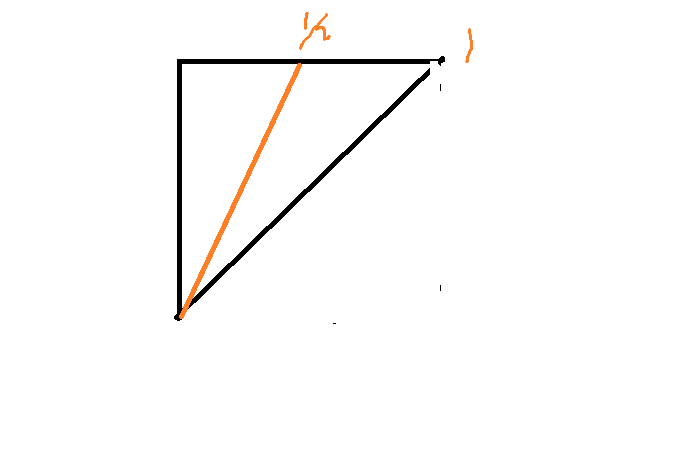
\includegraphics[width=3in]{hw09_3a.png}	
\end{figure}



\begin{align*}
	P(Y > 2X) &= \int_{0}^{\frac{1}{2}}\int_{2x}^{1} 90(y-x)^{8}dydx \\
	&= \int_{0}^{\frac{1}{2}}  \frac{90}{9} (y-x)^{9} \vert_{2x}^{1} dx \\
	&= \int_{0}^{\frac{1}{2}} 10 [(1-x)^{9}  - (x^{9})]dx \\
	&= \int_{0}^{\frac{1}{2}} 10 (1-x)^{9} dx - \int_{0}^{\frac{1}{2}} 10 x^{9}dx \\
	&= -(1-x)^{10} \vert_{0}^{\frac{1}{2}} - x^{10} \vert_{0}^{\frac{1}{2}} \\
	&= -\frac{1}{2}^{10} + 1^{10} - \frac{1}{2}^{10} \\
	&=  1 - 2(\frac{1}{2}^{10})\\
	&= 1 - 2 \cdot \frac{1}{2} (\frac{1}{2}^{9}) \\
	&= 1 - \left( \frac{1}{2} \right) ^{9} \\
\end{align*}




\textbf{b)} Find the marginal density of \(X\) and remember to provide
the possible values. Recognize the density as a member of a famous
family and state its name and parameters.

\begin{align*}
	f_{X}(x) &= \int_{Y} 90(y-x)^{8} dy \\
	&= \int_{x}^{1} 90(y-x)^{8} dy \\
	&= 10(y-x)^{9} \vert_{x}^{1} \\
	&= 10(1-x)^{9} , 0<x<1\\
\end{align*}

This is the Beta(1,10) distribution. 


\textbf{c)} Fill in the blanks (\textbf{prove your answer}): The joint
density \(f\) above is the joint density of the minimum and maximum of
ten independent uniform \((0, 1)\) random variables.
{[}Follow the steps in
\href{https://data140.org/textbook/content/chapter-17/beta-densities-with-integer-parameters/\#joint-density-of-two-order-statistics}{this
calculation} in the textbook.{]}



So we have 10 independent uniform(0,1) random variables. The density function is saying we have 0 r.vs in the interval between 0 and y (y terms), 8 of the uniform r.vs in the interval between y and x (y-x terms), and 0 of the r.v.s in the interval after x (1-x terms). Then, we have the last two uniform rvs in the areas around y and x (dy and dx). 
    \newpage

    \subsection{4. Peter Meets Paul}\label{peter-meets-paul}

Peter and Paul agree to meet at a restaurant at noon. Peter arrives at
time normally distributed with mean 12:00 noon and SD 3 minutes. Paul
arrives at a time normally distributed with mean 12:02 P.M. and SD 4
minutes.

Find the chances below assuming that the two arrival times are
independent.

\begin{itemize}
\tightlist
\item
  First, write a formula for the chance in terms of the standard normal
  cdf \(\Phi\).
\item
  Then use a code cell to find the numerical value. You do not have to
  turn in any coding work for this question.
\end{itemize}

Let Peter = X, Paul = Y

$ X \sim norm(0, 3), Y \sim norm(2, 4) $ 

\textbf{a)} \(P\)(Peter arrives before Paul)

\begin{align*}
	P(\text{Peter arrives before Paul}) &= P(X < Y) \\
	&= P(X - Y < 0) \\
	&= \Phi\left( \frac{(0- (-2)}{\sqrt{3^{2} + 4^{2}}} \right)  \\
&= \Phi\left( \frac{2}{5} \right)  \\
\approx 0.6554
\end{align*}


\textbf{b)} \(P\)(both men arrive within 3 minutes of noon)


\begin{align*}
	P(\text{both men arrive within 3 minutes of noon}) &= P(|X| \le 3, |Y| \le 3) \\
	&= P(|X| \le 3) P(|Y| \le 3) \\
	&= P(-3 \le X \le 3) P(-3 \le Y \le 3) \\
	&= \left( \Phi(\frac{3-0}{3}) - \Phi(\frac{-3-0}{3}) \right) \cdot \left( \Phi(\frac{-3-2}{4}) - \Phi(\frac{3-2}{4}) \right)  \\
	&= (\Phi(1) - \Phi(-1)) \cdot ( \Phi(\frac{1}{4}) - \Phi(-\frac{5}{4})\\
	&\approx 0.3366 \\
\end{align*}

\textbf{c)} \(P\)(the two men arrive within 3 minutes of each other)


\begin{align*}
	P(\text{two men arrive within 3 minutes of each other}) &= P(|X - Y| \le 3) \\
	&= P(-3 \le X - Y \le 3) \\
	&= \Phi(\frac{3 - (-2)}{5}) - \Phi( \frac{-3 - (-2)}{5}) \\
	&= \Phi(1) - \Phi(-\frac{1}{5}) \\
	&\approx 0.4206
\end{align*}
    \begin{tcolorbox}[breakable, size=fbox, boxrule=1pt, pad at break*=1mm,colback=cellbackground, colframe=cellborder]
\prompt{In}{incolor}{ }{\boxspacing}
\begin{Verbatim}[commandchars=\\\{\}]
\PY{c+c1}{\PYZsh{} Calculation for a}
\PY{o}{stats.norm.cdf(2/5)}
\end{Verbatim}
\end{tcolorbox}

    \begin{tcolorbox}[breakable, size=fbox, boxrule=1pt, pad at break*=1mm,colback=cellbackground, colframe=cellborder]
\prompt{In}{incolor}{ }{\boxspacing}
\begin{Verbatim}[commandchars=\\\{\}]
\PY{c+c1}{\PYZsh{} Calculation for b}
\PY{o}{.}\PY{o}{.}\PY{o}{.}
\end{Verbatim}
\end{tcolorbox}

    \begin{tcolorbox}[breakable, size=fbox, boxrule=1pt, pad at break*=1mm,colback=cellbackground, colframe=cellborder]
\prompt{In}{incolor}{ }{\boxspacing}
\begin{Verbatim}[commandchars=\\\{\}]
\PY{c+c1}{\PYZsh{} Calculation for c}
\PY{o}{.}\PY{o}{.}\PY{o}{.}
\end{Verbatim}
\end{tcolorbox}

    \newpage

    \subsection{5. Rayleigh Facts and an
Application}\label{rayleigh-facts-and-an-application}

Let \(R\) have the Rayleigh density given by
\(f(r) ~ = ~ re^{-\frac{1}{2}r^2}\) for \(r > 0\).

Refer to
\href{https://data140.org/textbook/content/chapter-18/standard-normal-basics/\#variance}{Section
18.1} and
\href{https://data140.org/textbook/content/chapter-18/chi-squared-distributions/\#from-chi-squared-1-to-chi-squared-n}{Section
18.4} for ways in which this density arises.

The point of Parts \textbf{a} and \textbf{b} is for you \emph{not to
reinvent wheels}, and also for you to notice that math calculation can
be reduced by using probability facts. The probabilistic approach to
math is powerful, so please follow the approach in the instructions. We
will not give credit for other approaches.

\textbf{a)} Write \(E(R)\) as an integral but don't find its value yet.
Let \(Z\) be standard normal. You know the numerical value of the
variance of \(Z\). Write the variance of \(Z\) as an integral, compare
with your integral for \(E(R)\), and use the comparison to find the
value of \(E(R)\).

\begin{align*}
	E[R] &= \int_{0}^{\infty } r \cdot re^{-\frac{1}{2}r^{2}} dr \\
	&= \int_{0}^{\infty }r^{2} e^{-\frac{1}{2}r^{2}}dr \\
\end{align*}


\begin{align*}
\Var(Z) &= E[Z^{2}] - E[Z]^{2} \\
&= E[Z^{2}] \\
&= 1 \\
\end{align*}


\[
	E[Z^{2}] = \int_{-\infty}^{\infty} z^{2} \frac{1}{\sqrt{2\pi}} e^{-\frac{1}{2}z^{2}}dz
\]

\begin{align*}
	E[Z^{2}] &= 2 \int_{0}^{\infty } z^{2} \frac{1}{\sqrt{2\pi}} e^{-\frac{1}{2}z^{2}}dz \\
		 &= \sqrt{\frac{2}{\pi}} \int_{0}^{\infty } z^{2} e^{-\frac{1}{2}z^{2}}dz \\
\end{align*}

Therefore, 

\begin{align*}
	E[R] &= \frac{E[Z^{2}]}{\sqrt{2 / \pi}} \\
	     &= \frac{1}{\sqrt{\frac{2}{\pi}}} \\
	     &= \sqrt{\frac{\pi}{2}} \\
\end{align*}

\textbf{b)} Use properties of \(R^2\) to find \(E(R^2)\) without any
further integration, and hence find \(Var(R)\).

\begin{align*}
	E[R^{2}] &= E[X^{2} + Y^{2}], \quad \text{where X,Y standard normal r.v}\\
	&= E[X^{2}] + E[Y^{2}] \\
	&= 1 + 1 \\
	&= 2 \\
\end{align*}

\[
\Var(R) = 2 - \frac{\pi}{2}
\]


\textbf{c)} Suppose two shots are fired at a target. Assume each shot
hits with independent normally distributed coordinates, with the same
means and equal unit variances. Let \(D\) be the distance between the
point where the two shots strike. Find \(E(D)\) and \(Var(D)\).

{[}Your calculations will go faster if you remember that a normal
\((0, \sigma^2)\) variable can be written as \(\sigma Z\) where \(Z\) is
standard normal, and if you use Parts \textbf{a-b}.{]}


$ D = \sqrt{(X_1-X_2)^{2} + (Y_{1} - Y_{2})^{2}} $, where (X, Y) is the point where a shot hit the target. 


This can be rewritten as: $D = \sqrt{X^{2} + Y^{2}} $, where $ X $ and $ Y $ are the differences in x and y coordinates. 

Hence, $ X \sim norm(0, 2) = \sqrt{2}Z_{X} $, $ Y \sim norm(0,2) = \sqrt{2}Z_{Y} $.  

\begin{align*}
	D &= \sqrt{2Z^{2} + 2Z^{2}} \\
	  &= \sqrt{2} \sqrt{Z_{X}^{2} + Z_{Y}^{2}} \\
\end{align*}


\begin{align*}
	E[D] &= \sqrt{2}E[\sqrt{Z_{X}^{2} + Z_{Y}^{2}}] \\
	     &= \sqrt{2} E[R] \\
	     &= \sqrt{\pi} \\
\end{align*}

\begin{align*}
	\Var(D) &= 2 \Var(R) \\
	&= 4 - \pi \\
\end{align*}


    \subsection{Submission Instructions}\label{submission-instructions}

Many assignments throughout the course will have a written portion and a
code portion. Please follow the directions below to properly submit both
portions.

\subsubsection{Written Portion}\label{written-portion}

\begin{itemize}
\tightlist
\item
  Scan all the pages into a PDF. You can use any scanner or a phone
  using applications such as CamScanner. Please \textbf{DO NOT} simply
  take pictures using your phone.
\item
  Please start a new page for each question. If you have already written
  multiple questions on the same page, you can crop the image in
  CamScanner or fold your page over (the old-fashioned way). This helps
  expedite grading.
\item
  It is your responsibility to check that all the work on all the
  scanned pages is legible.
\item
  If you used \(\LaTeX\) to do the written portions, you do not need to
  do any scanning; you can just download the whole notebook as a PDF via
  LaTeX.
\end{itemize}

\subsubsection{Code Portion}\label{code-portion}

\begin{itemize}
\tightlist
\item
  Save your notebook using
  \texttt{File\ \textgreater{}\ Save\ and\ Checkpoint}.
\item
  Generate a PDF file using
  \texttt{File\ \textgreater{}\ Download\ As\ \textgreater{}\ PDF\ via\ LaTeX}.
  This might take a few seconds and will automatically download a PDF
  version of this notebook.

  \begin{itemize}
  \tightlist
  \item
    If you have issues, please post a follow-up on the general Homework
    9 Ed thread.
  \end{itemize}
\end{itemize}

\subsubsection{Submitting}\label{submitting}

\begin{itemize}
\tightlist
\item
  Combine the PDFs from the written and code portions into one PDF.
  \href{https://smallpdf.com/merge-pdf}{Here} is a useful tool for doing
  so.
\item
  Submit the assignment to Homework 9 on Gradescope.
\item
  \textbf{Make sure to assign each page of your pdf to the correct
  question.}
\item
  \textbf{It is your responsibility to verify that all of your work
  shows up in your final PDF submission.}
\end{itemize}

If you are having difficulties scanning, uploading, or submitting your
work, please read the
\href{https://edstem.org/us/courses/94054/discussion/7533569}{Ed Thread}
on this topic and post a follow-up on the general Homework 9 Ed thread.

\subsection{\texorpdfstring{\textbf{We will not grade assignments which
do not have pages selected for each
question.}}{We will not grade assignments which do not have pages selected for each question.}}\label{we-will-not-grade-assignments-which-do-not-have-pages-selected-for-each-question.}


    % Add a bibliography block to the postdoc
    
    
    
\end{document}
